\documentclass[]{article}

% Imported Packages
%------------------------------------------------------------------------------
\usepackage{amssymb}
\usepackage{amstext}
\usepackage{amsthm}
\usepackage{amsmath}
\usepackage{enumerate}
\usepackage{fancyhdr}
\usepackage[margin=1in]{geometry}
\usepackage{graphicx}
\usepackage{extarrows}
\usepackage{setspace}
\usepackage{float}
%------------------------------------------------------------------------------

% Header and Footer
%------------------------------------------------------------------------------
\pagestyle{plain}
\renewcommand\headrulewidth{0.4pt}
\renewcommand\footrulewidth{0.4pt}
%------------------------------------------------------------------------------

% Title Details
%------------------------------------------------------------------------------
\title{
  Erudite\\
  \large \emph{An educational content management system}\\
  \vspace{1em}
  High-Level Architectural Design
}
\author{
  SE 3A04: Software Design II -- Large System Design
  \\
  \begin{tabular}{ l l }
    Kelvin Lin*   & STUDENT-NUM \\
    Danish Khan   & STUDENT-NUM \\
    Puru Jetly    & STUDENT-NUM \\
    Terrance Yip  & STUDENT-NUM \\
    Varun Hooda   & STUDENT-NUM \\
  \end{tabular}
}
\date{}
%------------------------------------------------------------------------------

% Document
%------------------------------------------------------------------------------
\begin{document}

\maketitle
\newpage

\tableofcontents
\newpage

\section{Introduction}
\label{sec:introduction}
This section outlines the purpose and provides a system description of the
Erudite project; along with an overview of the contents and organization of
this high-level architectural design document.


\subsection{Purpose}
\label{sub:purpose}
The purpose of this document to define the use cases, layout the Analysis Class
Diagram, describe the Architectural Design, and finally document the class
responsibilities through collaboration cards. This document builds on top of
and extends the Software Requirements Specification document in that this
document describes the way in which the system will interact with the outside
world and how the subsystems will be architecturally and logically arranged.

The target audience for this document are the stakeholders (Dr. Ridha Khedri,
Andrew Le Clair and Michael Liut), and any current or future architects,
designers and developers of this project.


\subsection{System Description}
\label{sub:system_description}
The Erudite application is intended to be an educational content management
system for use in elementary school classrooms. The primary interface between
the user and the software system is through a device running the Android
operating system. This document defines the way in which the users will be
expected to interact with the system and how the application will be decomposed
into smaller subsystems to reduce the complexity and improve the
maintainability, flexibility of this system.

Specifically, the users of this system (application) are expected to perform a
set of events that will prompt the system to react. The decomposition will then
show how the subsystems will communicate among one another in order to
efficiently distribute the work and perform the required actions in response to
the user's actions.


\subsection{Overview}
\label{sub:overview}
The remainder of the document is organized into 4 sections: Use Case Diagram --
how the users and system will interact, Analysis Class Diagram -- the
subsystems that compose this entire application, Architectural Design -- the
layout of the subsystems into a well-understood software architecture, and
Class responsibility collaboration Cards -- description of the interactions
between the subsystems. Each section uses an appropriate notation and diagrams
to document the design decision and describe the details of the high-level
design of this system.


% End Section


\newpage

\section{Use Case Diagram}
\label{sec:use_case_diagram}
% Begin Section
The following diagram is an use case diagram for Erudite.\\

{
\begin{figure}[h]
  \centering
  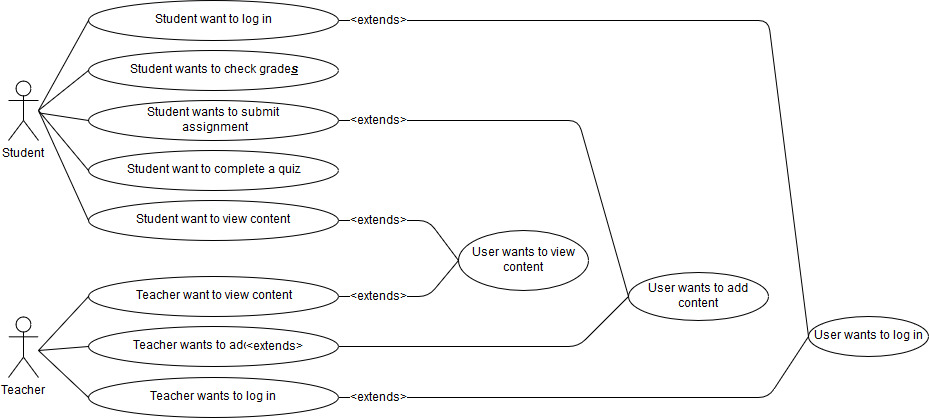
\includegraphics[scale=0.40]{A2_Assets/Use_Case_Diagram_v1.jpg}
  \caption{Use Case Diagram}
\end{figure}
}

\newpage

\section{Analysis Class Diagram}
\label{sec:analysis_class_diagram}
% Begin Section
The following diagram is an analysis class diagram for Erudite.\\

{
\begin{figure}[h]
  \centering
  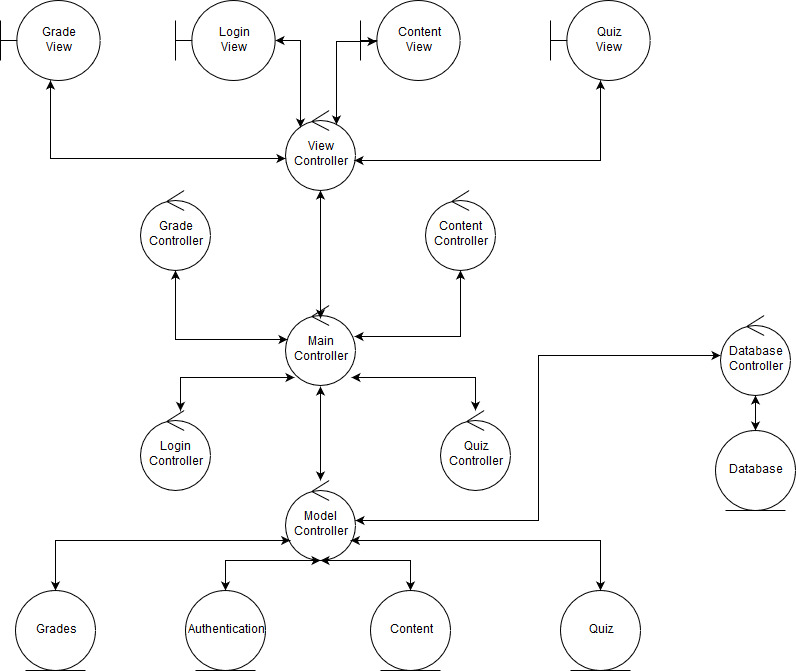
\includegraphics[scale=0.5]{A2_Assets/Analysis_Class_Diagrm_v2.jpg}
  \caption{Analysis Class Diagram}
\end{figure}
}


\section{Architectural Design}
\label{sec:architectural_design}
% Begin Section




\subsection{System Architecture}
\label{sub:system_architecture}
% Begin SubSection
Erudite will be built following the PAC architecture, where the system will be 
decomposed into a hierarchy of control modules, abstraction modules, and 
presentation modules.

The PAC architecture was chosen because Erudite is composed with multiple 
subsystems with interactive requirements. Each subsystem requires a view to 
display information, data which it processes for different users, and a 
controller to determine the sequence of events.

The main advantages of choosing the PAC architecture is it separates the 
different subsystems, and this allows for different people to implement the 
different subsystems independently of each other. Moreover, each component of 
the subsystem can also be separated so that each component can be implemented 
independently of each other.

Furthermore, the PAC architecture allows for high cohesion and low coupling 
systems. The PAC architecture ensures high cohesion because each subsystem can 
only interact with the related components, and the main controller. This ensures 
that only relevant components are grouped together, and other components are 
grouped in other subsystems. Moreover, each of the systems only has a single 
connection to the main controller, and not to any other subsystems. Aside from 
the main controller, all of the subsystems are loosely coupled with each other, 
and the internal implementation of each subsystem can be changed with minimal 
modifications to the other subsystems.

Finally, the main controller in the PAC architecture allows Erudite to be 
extensible. New features can be added to the system with minimal modification: 
only a new Controller-Abstraction-Presentation needs to be added. Accordingly, 
Erudite will be based off the PAC architecture because of its ability to support 
multiple interactive subsystems while ensuring important software design 
principles such as high cohesion and low coupling.

%Add a structural architecture diagram here
{
  \begin{figure}[h]
  \centering
    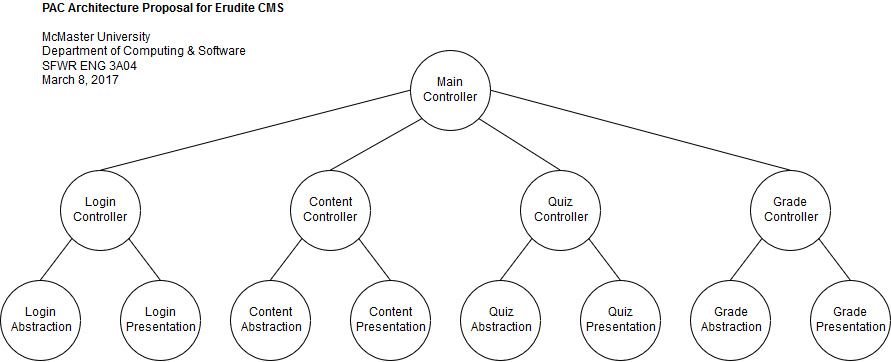
\includegraphics[scale=0.5]{A2_Assets/Structural_Class_Diagram_v3.jpg}
  \caption{Structural Architecture Diagram}
  \end{figure}
}
% End SubSection

\subsection{Subsystems}
\label{sub:subsystems}
% Begin SubSection
\subsubsection{The Main Control Subsystem}
The purpose of this subsystem is to determine when each of the other subsystems is active, and displays the active subsystem's view to the main view. It receives view information from each of the 4 subsystems, and it is responsible for routing information between different systems.

\subsubsection{The Content Management System}
The purpose of the content management system is to receive and display content to the users. It sends view information to the main controller to be displayed, and it receives messages from the main control system in order to determine when to activate. 

\subsubsection{The Quiz Management System}
The purpose of the quiz management system is to receive and display 
automated-evaluational content to the users. This system randomly selects 
multiple-choice questions from a question bank, shuffles answers and displays 
them to the user. It is connected to the main control system which dictates when this 
system is active, and it sends requests to the main control to be forwarded to 
 to the main view for display.

\subsubsection{The Grade Management System}
The grade management system is responsible for receiving and displaying student 
grades to the users according to user type. The system displays only grades 
relevant to the student if a student accesses grades and displays all assigned 
grades to a teacher should a teacher access course grades. This system is 
connected to the main control system which dictates when this system is active, and 
it sends requests to the main control to be forwarded to the main view for display.

\subsubsection{The Authentication System}
The authentication system authenticates the users' login credentials. This system is 
connected to the control system which dictates when this system is active, and 
it sends requests to the main control to be forwarded view for display.

% End SubSection

% End Section

\section{Class Responsibility Collaboration (CRC) Cards}
\label{sec:class_responsibility_collaboration_crc_cards}
% Begin Section
The tables below show the Class Responsibility Collaboration cards for Erudite.
	
	 %New CRC
	
	%Main view
	\begin{table}[H]
	\centering
		\begin{tabular}{|p{9cm}|p{3cm}|}
		\hline
		 \multicolumn{2}{|l|}{\textbf{Class Name: Main View}} \\
		\hline
		\textbf{Responsibility:} & \textbf{Collaborators:} \\
		\hline
	    Display Login View & Login View, Login Controller, Main Controller\\
		\hline
		Display Content View & Content View, Content Controller, Main Controller 	\\
		\hline
		Display Quiz View & Quiz View, Quiz Controller, Main Controller\\
		\hline
		Display Grade View & Grade View, Grade Controller, Main Controller\\
		\hline 
		Displays data from Main Controller & Main Controller\\
		\hline
		Send content response to Main Controller & Main Controller\\
		\hline
		\end{tabular}
	\end{table}	
	
	%Main Controller
	\begin{table}[H]
	\centering
		\begin{tabular}{|p{9cm}|p{3cm}|}
		\hline
		 \multicolumn{2}{|l|}{\textbf{Class Name: Main Controller}} \\
		\hline
		\textbf{Responsibility:} & \textbf{Collaborators:} \\
		\hline
	    Receive request to validate login credentials & Login Controller\\
		\hline
	    Handle login validation requests & Main Abstraction\\
		\hline
		Receive authentication status information & Main Abstraction\\
		\hline
		Forward authentication status information & Login Controller\\
		\hline
		Receive request for quiz questions & Quiz Controller\\
		\hline
		Retrieve quiz questions & Main Abstraction \\
		\hline
		Receive quiz questions & Main Abstraction\\
		\hline
		Forward quiz questions & Quiz Controller\\
		\hline
		Receive quiz submission & Quiz Controller\\
		\hline
		Send request to grade quiz submission & Main Abstraction\\
		\hline
		Receive quiz results & Main Abstraction\\
		\hline
		Forward status code to indicate submission status & Quiz Controller\\
		\hline
		Receive content & Main Abstraction\\
		\hline
		Forward content & Content Controller\\
		\hline
		Forward user submitted content for storage & Main Abstraction\\
		\hline
		Receive request for user grades & Grade Controller\\
		\hline
		Receive user grades & Main Abstraction\\
		\hline
		Forward user grades & Grade Controller\\
		\hline
		\end{tabular}
	\end{table}
	
	%Main Abstraction
	\begin{table}[H]
	\centering
		\begin{tabular}{|p{9cm}|p{3cm}|}
		\hline
		 \multicolumn{2}{|l|}{\textbf{Class Name: Main Abstraction}} \\
		\hline
		\textbf{Responsibility:} & \textbf{Collaborators:} \\
		\hline
		Know how to access central data repository & Void\\
		\hline
		\end{tabular}
	\end{table}
	
	 %login view
	\begin{table}[H]
	\centering
		\begin{tabular}{|p{9cm}|p{3cm}|}
		\hline
		 \multicolumn{2}{|l|}{\textbf{Class Name: Login View}} \\
		\hline
		\textbf{Responsibility:} & \textbf{Collaborators:} \\
		\hline
		Request username and password pair from user & Login Controller\\
		\hline
		Receive authentication status & Logic Controller\\
		\hline
		Display authentication status & Void\\
		\hline
		\end{tabular}
	\end{table}
	
	 %login controller
	\begin{table}[H]
	\centering
		\begin{tabular}{|p{9cm}|p{3cm}|}
		\hline
		 \multicolumn{2}{|l|}{\textbf{Class Name: Login Controller}} \\
		\hline
		\textbf{Responsibility:} & \textbf{Collaborators:} \\
		\hline
	    Refactor login credentials & Login Abstraction\\
		\hline
		Forward authentication request for verification & Main Controller\\
		\hline
		Relay authentication status to the view & Login View\\
		\hline
		\end{tabular}
	\end{table}
	
	 %login abstraction
	\begin{table}[H]
	\centering
		\begin{tabular}{|p{9cm}|p{3cm}|}
		\hline
		 \multicolumn{2}{|l|}{\textbf{Class Name: Login Abstraction}} \\
		\hline
		\textbf{Responsibility:} & \textbf{Collaborators:} \\
		\hline
	    Know how to represent a user's username & Void\\
		\hline
		Know how to represent a user's password & Void\\
		\hline
		Know how to represent a username/password pair & Void\\
		\hline
		\end{tabular}
	\end{table}
	
	 %quiz view
	\begin{table}[H]
	\centering
		\begin{tabular}{|p{9cm}|p{3cm}|}
		\hline
		 \multicolumn{2}{|l|}{\textbf{Class Name: Quiz view}} \\
		\hline
		\textbf{Responsibility:} & \textbf{Collaborators:} \\
		\hline
		Request quiz questions & Quiz Controller\\
		\hline
	    Receive quiz questions & Quiz Controller\\
	    \hline
	    Display quiz questions & Void\\
	    \hline 
	    Request user attempt & Quiz Controller\\
	    \hline
	    Request to submit quiz from user& Quiz Controller\\
	    \hline
	    Receive submission status & Quiz Controller\\
	    \hline
	    Display submission status & Void\\
	    \hline
		\end{tabular}
	\end{table}
	
	 %quiz controller
	\begin{table}[H]
	\centering
		\begin{tabular}{|p{9cm}|p{3cm}|}
		\hline
		 \multicolumn{2}{|l|}{\textbf{Class Name: Quiz Controller}} \\
		\hline
		\textbf{Responsibility:} & \textbf{Collaborators:} \\
		\hline
	    Refactor quiz questions & Quiz Abstraction\\
		\hline
		Refactor submission notification & Quiz Abstraction\\
		\hline
	    Send request for quiz questions & Main Controller\\
		\hline
		Receive quiz questions & Main Controller\\
		\hline
		Forward quiz questions & Quiz View\\
		\hline
		Send quiz submission notification & Main Controller\\
		\hline
		Receive submission status & Main Controller\\
		\hline
		Forward submission status & Quiz View\\
		\hline
		\end{tabular}
	\end{table}
	
	 %quiz abstraction
	\begin{table}[H]
	\centering
		\begin{tabular}{|p{9cm}|p{3cm}|}
		\hline
		 \multicolumn{2}{|l|}{\textbf{Class Name: Quiz Abstraction}} \\
		\hline
		\textbf{Responsibility:} & \textbf{Collaborators:} \\
		\hline
	    Know how to represent quiz questions  & Void\\
		\hline
		Know how to represent quiz submission & Void\\
		\hline
		\end{tabular}
	\end{table}

	%Content view
	\begin{table}[H]
	\centering
		\begin{tabular}{|p{9cm}|p{3cm}|}
		\hline
		 \multicolumn{2}{|l|}{\textbf{Class Name: Content View}} \\
		\hline
		\textbf{Responsibility:} & \textbf{Collaborators:} \\
		\hline
		Receive request for content from user & Content Controller\\
		\hline
	    Receive content & Content Controller\\
	    \hline
	    Display content & Void\\
	    \hline 
	    Receive request for formatted content from user & Content Controller\\
	    \hline
	    Receive file submissions from the user & Content Controller\\
	    \hline
	    Receive formatted content & Content Controller\\
	    \hline
	    Display formatted content & Void\\
	    \hline
		\end{tabular}
	\end{table}
	
	 %Content controller
	\begin{table}[H]
	\centering
		\begin{tabular}{|p{9cm}|p{3cm}|}
		\hline
		 \multicolumn{2}{|l|}{\textbf{Class Name: Content Controller}} \\
		\hline
		\textbf{Responsibility:} & \textbf{Collaborators:} \\
		\hline
	    Refactor content & Content Abstraction\\
		\hline
		Refactor formatted content & Content Abstraction\\
		\hline
	    Send request for content & Main Controller\\
		\hline
		Receive content & Main Controller\\
		\hline
		Forward content & Content View\\
		\hline
		Forward formatted content & Content View\\
		\hline
		Forward user submissions & Main Controller\\
		\hline	
		\end{tabular}
	\end{table}
	
	 %Content abstraction
	\begin{table}[H]
	\centering
		\begin{tabular}{|p{9cm}|p{3cm}|}
		\hline
		 \multicolumn{2}{|l|}{\textbf{Class Name: Content Abstraction}} \\
		\hline
		\textbf{Responsibility:} & \textbf{Collaborators:} \\
		\hline
	    Know how to represent content  & Void\\
		\hline
		Know how to represented formatted content & Void\\
		\hline
		\end{tabular}
	\end{table}
	
	%Grade view
	\begin{table}[H]
	\centering
		\begin{tabular}{|p{9cm}|p{3cm}|}
		\hline
		 \multicolumn{2}{|l|}{\textbf{Class Name: Grade View}} \\
		\hline
		\textbf{Responsibility:} & \textbf{Collaborators:} \\
		\hline
		Request user grades and statistics & Grade Controller\\
		\hline
	    Receive user grades and statistics & Grade Controller\\
	    \hline
	    Display user grades and statistics& Void\\
	    \hline 
		\end{tabular}
	\end{table}
	
	 %Grade controller
	\begin{table}[H]
	\centering
		\begin{tabular}{|p{9cm}|p{3cm}|}
		\hline
		 \multicolumn{2}{|l|}{\textbf{Class Name: Grade Controller}} \\
		\hline
		\textbf{Responsibility:} & \textbf{Collaborators:} \\
		\hline
	    Refactor grades & Grade Abstraction\\
		\hline
		Refactor grade statistics & Grade Abstraction\\
		\hline
	    Request user grades & Main Controller\\
		\hline
		Receive user grades & Main Controller\\
		\hline
		Forward user grades & Grade View\\
		\hline
		Forward user grades statistics & Grade View\\
		\hline
		\end{tabular}
	\end{table}
	
	 %Grade abstraction
	\begin{table}[H]
	\centering
		\begin{tabular}{|p{9cm}|p{3cm}|}
		\hline
		 \multicolumn{2}{|l|}{\textbf{Class Name: Grade Abstraction}} \\
		\hline
		\textbf{Responsibility:} & \textbf{Collaborators:} \\
		\hline
	    Know how to represent grades  & Void\\
		\hline
		Know how to represent quiz statistics & Void\\
		\hline
		\end{tabular}
	\end{table}

% End Section

\newpage
\appendix
\section{Division of Labour}
\label{sec:division_of_labour}
\begin{description}
  \item [Kelvin Lin ]
  \item{Section 4.1}
  \item{Section 4.2}
  \item{General editing and formatting}
  \hfill \rule{2in}{0.1pt}
  \\\\

  \item [Danish Khan]
  \item{CRC Cards}
  \item{Structural Class Diagram}
  \hfill \rule{2in}{0.1pt}
  \\\\

  \item [Puru Jetly]
  \item{CRC Cards}
  \item{General editing and formatting}
  \hfill \rule{2in}{0.1pt}
  \\\\

  \item [Terrance Yip]
   \item{CRC Cards}
  \item{Analysis Class Diagram}
  \hfill \rule{2in}{0.1pt}
  \\\\

  \item [Varun Hooda]
  \item{Section 1 Introduction}
  \item{Revision to use case diagram}
  \hfill \rule{2in}{0.1pt}
  \\\\
\end{description}

\newpage
\section{Apportioning of Requirements}
The following business events will not be addressed in the future deliverables.

\begin{enumerate}[{BE}1.]
	\item A teacher wants to create a course.
	\begin{enumerate}[{VP1}.1]
		\item Student Viewpoint
			\begin{enumerate}
				\item Students shall be able to enrol in an existing course owned by the
teacher provided the course is set visible.
			\end{enumerate}
		\item Teacher Viewpoint
			\begin{enumerate}
			    \item The teacher shall own the created course.
				\item A teacher shall be able to choose to unenroll a student from a course
that the teacher owns.
				\item A teacher shall not be enrolled in a course.
			\end{enumerate}
		\item Parent Viewpoint
			\begin{enumerate}
				\item Parents shall be able to view the course's progress or student
performance through their child's account.
			\end{enumerate}
		\item School Administration Viewpoint
			\begin{enumerate}
				\item The school administration shall be allowed to choose to whether to
allow students and teachers
to create their own accounts, or create accounts for all students and teachers.
			\end{enumerate}
		\item Information Technology Team Viewpoint
			\begin{enumerate}
				\item None
			\end{enumerate}
		\item Government \& School Board Viewpoint
			\begin{enumerate}
				\item All courses, course content, student content and any teacher student
communication held on the on the system shall be made visible to the school
board.
			\end{enumerate}
	\end{enumerate}

	\item A teacher wants to add content to a course they own.
	\begin{enumerate}[{VP1}.1]
		\item Student Viewpoint
			\begin{enumerate}
        \item A student enrolled in a course shall be able to view any content 
within the course when the content is set visible by the owner of that course.
        \item The system shall provide interface elements that allow the student 
to view any content set visible by the course owner.
        \item A student shall be able to submit an \underline{assignment}; a 
piece of content uploaded in response to a manual-evaluational content when the 
manual-evaluational content is set visible by the owner of that course and file 
submission is enabled.
        \item The system shall provide interface elements that allow the student 
to submit an assignment in response to manual-evaltional content.
        \item A student shall be able to submit an automated-evaluational 
content when it is set visible by the owner of that course.
        \item The system shall provide interface elements that allow the student 
to open and submit automated-evaluational content that is set visible by the 
owner of the course.
			\end{enumerate}
		\item Teacher Viewpoint
			\begin{enumerate}
				\item Teachers shall be allowed to set permissions that students have over 
each file.
        \item The system shall provide interface elements that allow the teacher 
to set permissions that students have over each file.
				\item The teacher shall specify a time period for which file submission is 
accepted by the manual-evaluational piece of content for manual-evaluational 
content.
        \item The system shall provide interface elements that allow the teacher 
to speicify the time period for which file submission is accepted by 
manual-evaluational content.
			\end{enumerate}
		\item Parent Viewpoint
			\begin{enumerate}
				\item None
			\end{enumerate}
		\item School Administration Viewpoint
			\begin{enumerate}
				\item None
			\end{enumerate}
		\item Information Technology Team Viewpoint
			\begin{enumerate}
				\item None
			\end{enumerate}
		\item Government \& School Board Viewpoint
			\begin{enumerate}
				\item None
			\end{enumerate}
	\end{enumerate}

	\item A teacher wants to add automated-evaluational content.
	\begin{enumerate}[{VP2}.1]

		\item Student Viewpoint
			\begin{enumerate}
        \item Students shall be able to view the automated-evaluational content
          only if the teacher sets the visibility of the content to be viewable
          by students.

        \item Students shall be able to open automated-evaluational content for
          a predefined period of time specified by the course owner when the
          content is made visible.

        \item Automated-evaluational content that has been opened and viewed by
          a student shall be submitted manually by the student or automatically
          before or at the end of predefined time (as specified by the teacher)
          respectively.
			\end{enumerate}

		\item Teacher Viewpoint
			\begin{enumerate}
        \item The teacher shall specify the visibility of the
          automated-evaluational content or it will default to "not visible to
          students".
			\end{enumerate}

		\item Parent Viewpoint
			\begin{enumerate}
				\item None
			\end{enumerate}

		\item School Administration Viewpoint
			\begin{enumerate}
				\item None
			\end{enumerate}

		\item Information Technology Team Viewpoint
			\begin{enumerate}
				\item None
			\end{enumerate}

		\item Government \& School Board Viewpoint
			\begin{enumerate}
				\item None
			\end{enumerate}

	\end{enumerate}

  \item The owner of a course specifies a time period in which non-evaluational
    content, manual-evaluational content, automated-evaluational content or a
    course is set visible for all enrolled students.
	\begin{enumerate}[{VP2}.1]

		\item Student Viewpoint
			\begin{enumerate}
        \item Students shall be unenrolled from a course that is set to not
          visible.

        \item Students shall not be able to view a course or
          \textbf{course content} which is not made visible to them.
			\end{enumerate}

		\item Teacher Viewpoint
			\begin{enumerate}
        \item The teacher shall be able to permanently remove \textbf{course
          content} from a course owned by them.
			\end{enumerate}

		\item Parent Viewpoint
			\begin{enumerate}
				\item None
			\end{enumerate}

		\item School Administration Viewpoint
			\begin{enumerate}
				\item None
			\end{enumerate}

		\item Information Technology Team Viewpoint
			\begin{enumerate}
				\item None
			\end{enumerate}

		\item Government \& School Board Viewpoint
			\begin{enumerate}
				\item None
			\end{enumerate}
	\end{enumerate}

  \item A student attempts to enroll in a course.
	\begin{enumerate}[{VP2}.1]
		\item Student Viewpoint
			\begin{enumerate}
        \item A student shall not be able to enroll in a course that is not
          visible to them.
        \item A student shall be able view all courses in which they are
          enrolled.
        \item A student shall not be able to self withdraw from a course in
          which he or she is enrolled.
        \item A student that is dismissed from a course shall no longer be
          enrolled in that course.
        \item A dismissed student shall not self enroll in a course from which
          he or she was dismissed.
        \item A student whom is not enrolled in a course shall have no access
          to \textbf{course content} found within that course.
			\end{enumerate}
		\item Teacher Viewpoint
			\begin{enumerate}
        \item A teacher shall be able to dismiss an enrolled student from a
          course owned by that teacher.
			\end{enumerate}
		\item Parent Viewpoint
			\begin{enumerate}
				\item None
			\end{enumerate}
		\item School Administration Viewpoint
			\begin{enumerate}
        \item The school administration shall be able to dismiss an enrolled
          student from a course.
			\end{enumerate}
		\item Information Technology Team Viewpoint
			\begin{enumerate}
				\item None
			\end{enumerate}
		\item Government \& School Board Viewpoint
			\begin{enumerate}
				\item None
			\end{enumerate}
	\end{enumerate}


	\item The school administration wants to add a Teacher or a Student account.
	\begin{enumerate}[{VP1}.1]
		\item Student Viewpoint
			\begin{enumerate}
				\item The student shall receive a Student ID and password to access their
personal if a new student account.
				\item The system shall allow the student to access their personal account 
when given the correct student id and password.
				\item The student shall choose a new password upon first signing into the
system.
				\item The system shall prompt new users to change their password.
			\end{enumerate}
		\item Teacher Viewpoint
			\begin{enumerate}
				\item The teacher shall receive a Teacher ID and password to access their
personal teacher account.
				\item The system shall allow a teacher to access their personal account 
given the correct login credentials.
				\item The teacher shall choose a new password upon first signing into the
system.
				\item The system shall prompt new users to change their password.
			\end{enumerate}
		\item Parent Viewpoint
			\begin{enumerate}
				\item None
			\end{enumerate}
		\item School Administration Viewpoint
			\begin{enumerate}
				\item The School Administration shall be able to create a set of usernames
and passwords from an external file.
				\item The system shall store a set of usernames and passwords.
			\end{enumerate}
		\item Information Technology Team Viewpoint
			\begin{enumerate}
				\item None
			\end{enumerate}
		\item Government \& School Board Viewpoint
			\begin{enumerate}
				\item The school administration shall monitor communication.
				\item The system shall provide functionality for the school administration 
to monitor communication
				\item All enquiries shall be
forwarded to the school administration.
				\item The system shall forward all enquiries to the school administration.
				\item The school
administration shall be given access and privileges to hide, remove or track the
origin of a piece of content or course when any content malign against board
policies is uploaded to the system.
				\item The system shall have privileges that are provided to the school 
administration to remove and track origins of a piece of content or course.
			\end{enumerate}
	\end{enumerate}

	\item The school administration wants to delete a course.
	\begin{enumerate}[{VP1}.1]
		\item Student Viewpoint
			\begin{enumerate}
				\item All students shall be unenrolled from the course.
				\item The system shall allow student to be unenrolled from courses.
			\end{enumerate}
		\item Teacher Viewpoint
			\begin{enumerate}
				\item A teacher shall not own a deleted course.
				\item The system shall check that no teachers have a deleted course.
				\item{All content shall be deleted from the system.}
				\item The system shall delete all the content from a deleted course.
			\end{enumerate}
		\item Parent Viewpoint
			\begin{enumerate}
				\item None
			\end{enumerate}
		\item School Administration Viewpoint
			\begin{enumerate}
				\item The school administration account shall be given a warning after a
course
deletion request is made.
				\item The system shall alert the school administration when deletion request 
is made.
\item The course shall deleted only if a course deletion
request is made a second time following the warning.
\item The system shall only allow the course to be deleted after another 
deletion request is made after the warning.
			\end{enumerate}
		\item Information Technology Team Viewpoint
			\begin{enumerate}
				\item None
			\end{enumerate}
		\item Government \& School Board Viewpoint
			\begin{enumerate}
				\item None
			\end{enumerate}
	\end{enumerate}
\end{enumerate}

% \newpage
% \section*{IMPORTANT NOTES}
% \begin{itemize}
%   \item You do \underline{NOT} need to provide a text explanation of each
%   diagram; the diagram should speak for itself
%   \item Please document any non-standard notations that you may have used
%   \begin{itemize}
%     \item \emph{Rule of Thumb}: if you feel there is any doubt surrounding
%     the meaning of your notations, document them
%   \end{itemize}
%   \item Some diagrams may be difficult to fit into one page
%   \begin{itemize}
%     \item It is OK if the text is small but please ensure that it is readable
%     when printed
%     \item If you need to break a diagram onto multiple pages, please adopt a
%     system of doing so and thoroughly explain how it can be reconnected from
%     one page to the next; if you are unsure about this, please ask about it
%   \end{itemize}
%   \item Please submit the latest version of Deliverable 1 with Deliverable 2
%   \begin{itemize}
%     \item It does not have to be a freshly printed version; the latest marked
%     version is OK
%   \end{itemize}
%   \item If you do \underline{NOT} have a Division of Labour sheet, your
%   deliverable will \underline{NOT} be marked
% \end{itemize}


\end{document}
%------------------------------------------------------------------------------




